% Exam Template using Philip Hirschhorn's exam.cls: http://www-math.mit.edu/~psh/#ExamCls
%
% run pdflatex on a finished exam at least three times to do the grading table on front page.
%
%%%%%%%%%%%%%%%%%%%%%%%%%%%%%%%%%%%%%%%%%%%%%%%%%%%%%%%%%%%%%%%%%%%%%%%%

% These lines can probably stay unchanged, although you can remove the last two packages if you're not making pictures with tikz.
\documentclass[12pt,legalpaper]{exam}
\RequirePackage{amssymb, amsfonts, amsmath, latexsym, verbatim, xspace, setspace, graphicx, enumerate, paralist, array}
\newcolumntype{L}[1]{>{\raggedright\let\newline\\\arraybackslash\hspace{0pt}}m{#1}}
\newcolumntype{C}[1]{>{\centering\let\newline\\\arraybackslash\hspace{0pt}}m{#1}}
\newcolumntype{R}[1]{>{\raggedleft\let\newline\\\arraybackslash\hspace{0pt}}m{#1}}

% By default LaTeX uses large margins.  This doesn't work well on exams; problems end up in the "middle" of the page, reducing the amount of space for students to work on them.
\usepackage[margin=1in]{geometry}


% Here's where you edit the Class, Exam, Date, etc.
\newcommand{\class}{Math 1070}
\newcommand{\term}{Winter 2024}
\newcommand{\examnum}{Final Exam}
\newcommand{\examdate}{April 20th}
\newcommand{\timelimit}{3 hours}


% For an exam, single spacing is most appropriate
\singlespacing
% \onehalfspacing
% \doublespacing

% For an exam, we generally want to turn off paragraph indentation
\parindent 0ex

\usepackage[dvipsnames, table]{xcolor}

\usepackage{
  amsmath,
  amssymb, 
  arydshln, % for hyphenated lines in block matrices
  graphicx, % to include pictures
  hyperref, % for hyper links
  mathtools, % for a longer arrow
  multicol, % displaying enumerates and itemizes into multiple columns
  multirow, % so that vertical lines aren't missing in the table at the beginning of the exam
  multido, % for TOC
  pgfplots, % for axis environment within tikz pictures
  systeme,
  tikz,
}

\usepackage[inline, shortlabels]{enumitem}

% mathbb aliases
\newcommand{\COMPLEX}{\mathbb{C}}
\newcommand{\REAL}{\mathbb{R}}
\newcommand{\NATURAL}{\mathbb{N}}
\newcommand{\INTEGER}{\mathbb{Z}}

% nicer looking trig functions
\newcommand{\SIN}[1]{\sin\left(#1\right)}
\newcommand{\COS}[1]{\cos\left(#1\right)}
\newcommand{\TAN}[1]{\tan\left(#1\right)}
\newcommand{\CSC}[1]{\csc\left(#1\right)}
\newcommand{\SEC}[1]{\sec\left(#1\right)}
\newcommand{\COT}[1]{\cot\left(#1\right)}

% automatically resize set brackets
\newcommand{\SET}[1]{\left\{#1\right\}}

% sums and products
\newcommand{\SUM}{\displaystyle\sum\limits}
\newcommand{\PROD}{\displaystyle\prod\limits}
\newcommand{\of}{\circ}
\newcommand{\restrict}[1]{\raisebox{-.5ex}{$|$}_{#1}}

% set intersection and union
\newcommand{\CAP}{\displaystyle\bigcap\limits}
\newcommand{\CUP}{\displaystyle\bigcup\limits}

% max and min
\newcommand{\MAX}[1]{\ensuremath{\max\left(#1\right)}}
\newcommand{\MIN}[1]{\ensuremath{\min\left(#1\right)}}

% for writing logic within mathematics environment
\newcommand{\FORALL}{\ensuremath{\text{ for all }}}
\newcommand{\FORSOME}{\ensuremath{\text{ for some }}}

% matrix notation
\newcommand{\MATRIX}[2]{\ensuremath{\left[\begin{array}{#1}#2\end{array}\right]}}
\newcommand{\COLUMN}[1]{\ensuremath{\left[\begin{array}{r}#1\end{array}\right]}}

% vector notation
%\newcommand{\vv}{\overset{\rightharpoonup}}
\newcommand{\vv}[1]{{\bf #1}}
\newcommand{\arr}{\overrightarrow}

% dot product
\newcommand{\dotp}{{\scriptstyle\bullet}}

% Text macros
\newcommand{\KER}[1]{\ensuremath{\text{ker}\left(#1\right)}}
\newcommand{\IMG}[1]{\ensuremath{\text{im}\left(#1\right)}}
\newcommand{\CHAR}[1]{\ensuremath{\text{char}\left(#1\right)}}
\newcommand{\BIGO}[1]{\ensuremath{\mathcal{O}\left(#1\right)}}
\newcommand{\TR}[1]{\ensuremath{\text{tr}\left(#1\right)}}

% abbreviations
\newcommand{\p}{\noindent}
\newcommand{\ds}{\displaystyle}
\newcommand{\md}{\mdseries}
\newcommand{\vsp}{\vspace{0.5cm}}
\newcommand{\smsp}{\vspace{0.25cm}}
\newcommand{\hsp}{\hspace{0.25cm}}

% new operators
\DeclareMathOperator\SPAN{Span}
\newcommand{\SPANOF}[1]{\ensuremath{\SPAN\left\{#1\right\}}}
\DeclareMathOperator\PROJ{proj}
\DeclareMathOperator\PERP{perp}

\begin{document} 

% These commands set up the running header on the top of the exam pages
\pagestyle{head}
\firstpageheader{}{}{}
\runningheader{\class}{\examnum\ - Page \thepage\ of \numpages}{\examdate}
\runningheadrule

\begin{flushright}
\begin{tabular}{p{3.8in} r l}
\textbf{\class} & \textbf{Full Name:} & \makebox[2in]{\hrulefill}\\
\textbf{\term} & \textbf{ID:} & \makebox[2in]{\hrulefill}\\
\textbf{\examnum} &&\\
\textbf{\examdate} &&\\
\textbf{Time Limit: \timelimit} &
\end{tabular}\\
\end{flushright}
\rule[1ex]{\textwidth}{.1pt}

\textbf{Reminders:} 
\begin{itemize}

\item \textbf{Clearly identify your final answer}, by circling it or enclosing it in a box.  It's fine if you run out of space and write on the back of the page, just be sure to write a note indicating you have done so.

\item \textbf{Unsupported answers may not receive full credit}.  A correct answer, unsupported by calculations, explanation,
or algebraic work may receive little or no credit; an incorrect answer supported by some correct calculations will likely receive partial credit.

\item \textbf{Organize your work}, in a reasonably neat and coherent way, in the space provided.  Work scattered all over the page without a clear ordering will receive very little credit.
\end{itemize}
\vsp

\addpoints

\noindent
\begin{center}
\gradetablestretch{2}
\vqword{Page}
\gradetable[v][pages]  % Use [pages] to have grading table by page instead of question
\end{center}


\newpage % End of cover page

%%%%%%%%%%%%%%%%%%%%%%%%%%%%%%%%%%%%%%%%%%%%%%%%%%%%%%%%%%%%%%%%%%%%%%%%%%%%%%%%%%%%%
%
% See http://www-math.mit.edu/~psh/#examCls for full documentation, but the questions
% below give an idea of how to write questions [with parts] and have the points
% tracked automatically on the cover page.
%
%
%%%%%%%%%%%%%%%%%%%%%%%%%%%%%%%%%%%%%%%%%%%%%%%%%%%%%%%%%%%%%%%%%%%%%%%%%%%%%%%%%%%%%

\begin{questions}


\question[5] Formulate the following as a linear programming problem.  \textbf{You do not need to solve the problem.}
\begin{quote}
Harvest Farms is planning their crop distribution of corn and wheat for the upcoming year.  They own a total of 20 acres of land, and have access to 30 units of water.  On average,
\begin{itemize}
\item each acre of corn requires requires 2 units of water and generates 5 thousand dollars in profit, and
\item each acre of what requires 3 units of water and generates 8 thousand dollars in profit.
\end{itemize}
How many acres of each crop should be planted in order to maximize profit?
\end{quote}
\begin{enumerate}[(a)]
\item Introduce variables, using complete sentences.  Be sure to include units!
\vspace{4cm}

\item What is the objective function?  Is it to be maximized or minimized?
\vspace{4cm}

\item Specify all constraints as a system of linear inequalities.
\newpage
\end{enumerate}

\question[5] Formulate the following as a linear programming problem.  \textbf{You do not need to solve the problem.}
\begin{quote}
The management team at Efficient Electronics produces smartphones and tablets.  Each smartphone produced will yield a profit of \$50, while each tablet produced will yield a profit of \$80.  On average,
\begin{itemize}
\item each smartphone requires 5 days of production time and 4 units of materials, and
\item each tablet requires 3 days of production time and 6 units of material.
\end{itemize}
Their factory has 400 units of production time and 600 units of materials available each month.  How many smartphones and tablets should they produce each month to maximize their profit?
\end{quote}
\begin{enumerate}[(a)]
\item Introduce variables, using complete sentences.  Be sure to include units!
\vspace{4cm}

\item What is the objective function?  Is it to be maximized or minimized?
\vspace{4cm}

\item Specify all constraints as a system of linear inequalities.
\newpage
\end{enumerate}

\question[5] Solve the following linear programming problem, using the Method of Corners.
\vsp

\p Maximize
\begin{center}
$P = 3x + 5y$,
\end{center}
subject to
\begin{center}
$\begin{cases}
2x + y\leq 12\\
x+5y\leq 15\\
x,y\geq 0
\end{cases}$.
\end{center}
\vsp
\vfill

\hfill
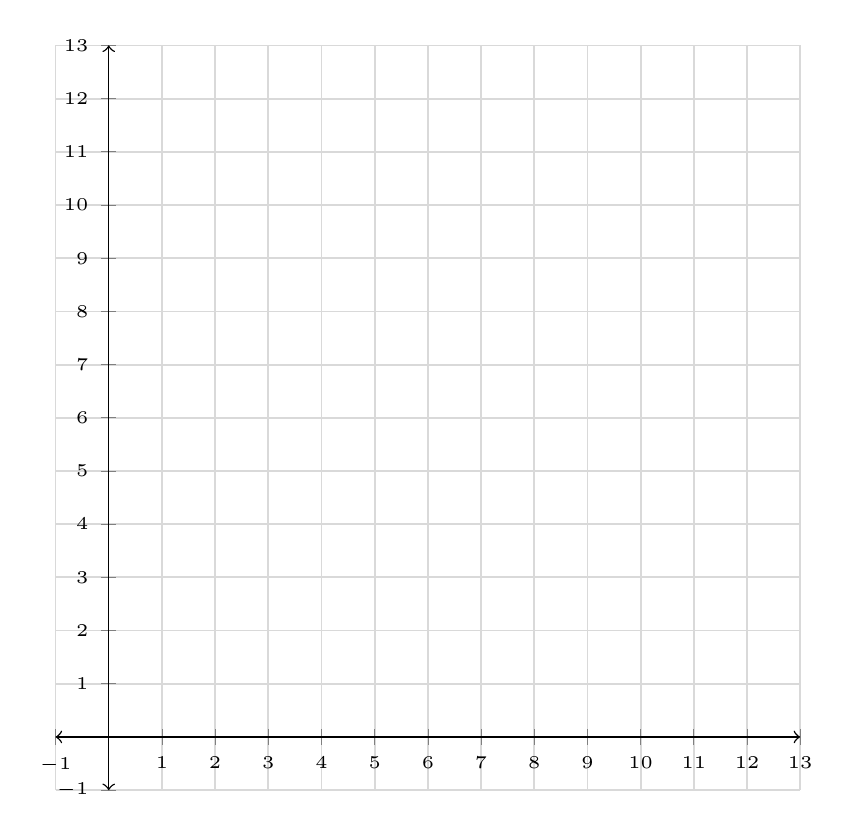
\begin{tikzpicture}[scale=1.3]
\begin{axis}[
  scale only axis,
  grid=both,
  grid style={line width=0.5pt, draw=gray!30},
    axis equal image,
    axis lines=middle,
    x axis line style={<->},
    y axis line style={<->},
    ticklabel style={font=\tiny},
    xtick distance=1,
    ytick distance=1,
    xmin=-1,
    xmax=13,
    ymin=-1,
    ymax=13,
    samples=50
]
\end{axis}
\end{tikzpicture}
\newpage

\question[5] Solve the following linear programming problem, using the Method of Corners.
\vsp

\p Maximize
\begin{center}
$P = 3x + 5y$,
\end{center}
subject to
\begin{center}
$\begin{cases}
2x + y\leq 8\\
x+2y\leq 10\\
x,y\geq 0
\end{cases}$.
\end{center}
\vsp
\vfill

\hfill
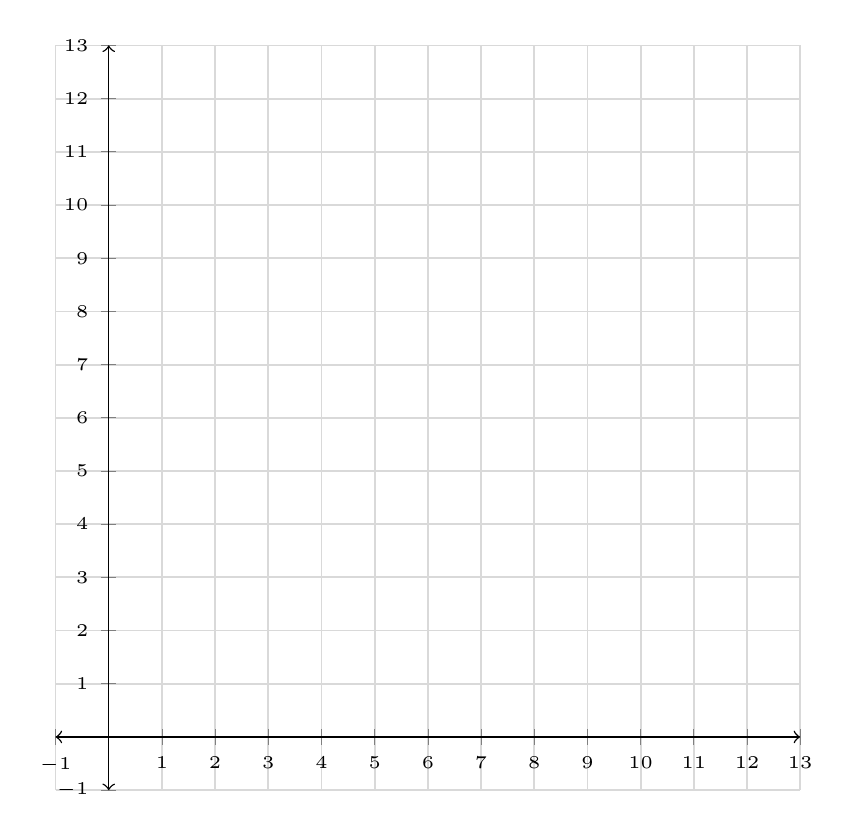
\begin{tikzpicture}[scale=1.3]
\begin{axis}[
  scale only axis,
  grid=both,
  grid style={line width=0.5pt, draw=gray!30},
    axis equal image,
    axis lines=middle,
    x axis line style={<->},
    y axis line style={<->},
    ticklabel style={font=\tiny},
    xtick distance=1,
    ytick distance=1,
    xmin=-1,
    xmax=13,
    ymin=-1,
    ymax=13,
    samples=50
]
\end{axis}
\end{tikzpicture}
\newpage

\question[5] Bob runs a shoe-store at a large retail mall.  Each month, he pays \$13,386.00 in rent, with average electric bills in the amount of \$870.00.  On average, his suppliers charge \$36.00 for a pair of shoes, and he sells each pair to customers for \$180.00.  Assume that Bob has no other costs to worry about.
\begin{compactenum}[(a)]
\item Find each of the revenue, cost, and profit functions for Bob's montly shoe sales.
\vspace{1cm}

\begin{itemize}
\item[] $R(q) =$
\vspace{1.5cm}

\item[] $C(q) =$
\vspace{1.5cm}

\item[] $P(q) =$
\end{itemize}
\vspace{1.5cm}

\fullwidth{\textbf{Be sure to answer the next question using at least one of the functions above.  Don't simply write down the answer, even if you find you are able to do it in your head.}}
\smsp

\item Assuming Bob's total costs are \$31,536.00, how many pairs of shoes did Bob order from his supplier?
\vfill

\item If Bob orders 124 pairs of shoes from his supplier, what is his total profit from selling them all?
\vfill

\item How many pairs of shoes must Bob sell each month in order to break even?
\vfill
\end{compactenum}
\newpage

\question[5] Jill runs a shoe-store at a large retail mall.  Each month, she pays \$14,990.00 in rent, with average electric bills in the amount of \$880.00.  On average, her suppliers charge \$32.00 for a pair of shoes, and she sells each pair to customers for \$170.00.  Assume that Jill has no other costs to worry about.
\begin{compactenum}[(a)]
\item Find each of the revenue, cost, and profit functions for Jill's montly shoe sales.
\vspace{1cm}

\begin{itemize}
\item[] $R(q) =$
\vspace{1.5cm}

\item[] $C(q) =$
\vspace{1.5cm}

\item[] $P(q) =$
\end{itemize}
\vspace{1.5cm} 

\fullwidth{\textbf{Be sure to answer the next question using at least one of the functions above.  Don't simply write down the answer, even if you find you are able to do it in your head.}}
\smsp

\item Assuming Jill's total costs are \$29,950.00, how many pairs of shoes did Jill order from her supplier?
\vfill

\item If Jill orders 39 pairs of shoes from her supplier, what is her total profit from selling them all?
\vfill

\item How many pairs of shoes must Jill sell each month in order to break even?
\vfill
\end{compactenum}
\newpage

\question[4] The supply and demand equations for a particular grocery store product are given by
\begin{center}
$\text{(Demand) }q = \sqrt{100 - p}$ and $\text{(Supply) }2q - p + 20 = 0$.
\end{center}
Find the equilibrium price $p_{0}$ and the equilibrium quantity $q_{0}$.
\vspace{15cm}

\question[3] Calculate the effective annual rate for each of the following interest plans.
\begin{compactenum}[(a)]
\item 5\% compounded continuously
\vspace{5cm}

\item 5.2\% compounded semi-annually
\vspace{5cm}
\end{compactenum}
\newpage

\question[5] A merchant observes on average, that
\begin{itemize}
\item 280 daily t-shirts will sell at \$19 each, and
\smsp

\item 268 daily t-shirts will sell at \$22 each.
\end{itemize}
\vsp

\begin{compactenum}[(a)]
\item Find the demand equation $p = D(q)$, assuming that $p$ and $q$ have a linear relationship.
\vspace{5cm}

\item Find the revenue function $R(q)$ as a function of quantity $q$ sold.
\vspace{8cm}

\item Find the number of t-shirts that should be sold daily to maximize the revenue.
\end{compactenum}
\newpage

\question[5] A merchant observes on average, that
\begin{itemize}
\item 240 daily t-shirts will sell at \$20 each, and
\smsp

\item 210 daily t-shirts will sell at \$25 each.
\end{itemize}
\vsp

\begin{compactenum}[(a)]
\item Find the demand equation $p = D(q)$, assuming that $p$ and $q$ have a linear relationship.
\vspace{5cm}

\item Find the revenue function $R(q)$ as a function of quantity $q$ sold.
\vspace{8cm}

\item Find the number of t-shirts that should be sold daily to maximize the revenue.
\end{compactenum}
\newpage

\question[5] Consider the difference equation $y_{n} = -0.5y_{n-1} + 6$ with $y_{0} = 13$.
\begin{compactenum}[(a)]
\item State whether this determines a monotonic or oscillating sequence, and why.
\vfill

\item What is the equilibrium value of this sequence?
\vfill

\item State whether this sequence is attracted to, or repelled by its equilibrium value.
\vfill

\item Sketch the sequence.
\vsp

\hfill
\begin{tikzpicture}[scale=1]
\begin{axis}[
%	grid=both,
%	axis equal image,
	%grid style={line width=0.5pt, draw=gray!30},
    scale only axis,
    axis lines=middle,
    x axis line style={->},
    y axis line style={<->},
    xtick distance=1,
    xticklabels={},
    yticklabels={},
    ymin=-7.5,
    ymax=22.5,
    xmin=0,
    xmax=6.5,
    samples=50
]
\end{axis}
\end{tikzpicture}

\item Solve the difference equation.
\vfill

\end{compactenum}
\newpage

\question[5] Consider the difference equation $y_{n} = -0.2y_{n-1} + 7.2$ with $y_{0} = 9$.
\begin{compactenum}[(a)]
\item State whether this determines a monotonic or oscillating sequence, and why.
\vfill

\item What is the equilibrium value of this sequence?
\vfill

\item State whether this sequence is attracted to, or repelled by its equilibrium value.
\vfill

\item Sketch the sequence.
\vsp

\hfill
\begin{tikzpicture}[scale=1]
\begin{axis}[
%	grid=both,
%	axis equal image,
	%grid style={line width=0.5pt, draw=gray!30},
    scale only axis,
    axis lines=middle,
    x axis line style={->},
    y axis line style={<->},
    xtick distance=1,
    xticklabels={},
    yticklabels={},
    ymin=-7.5,
    ymax=22.5,
    xmin=0,
    xmax=6.5,
    samples=50
]
\end{axis}
\end{tikzpicture}

\item Solve the difference equation.
\vfill

\end{compactenum}
\newpage

\question[4] A company has borrowed \$130,000.  The loan is to be repaid in monthly payments over 5 years.  Assume that the interest rate is 3\%, compounded weekly.
\begin{compactenum}[(a)]
\item Find the amount of each payment.
\vspace{10cm}

\item How much interest will be paid over the lifetime of this loan?
\vspace{8cm}

\item What will be the outstanding balance of of the loan after 3 years?
\end{compactenum}
\newpage

\question[4] A company has borrowed \$170,000.  The loan is to be repaid in monthly payments over 4 years.  Assume that the interest rate is 2\%, compounded weekly.
\begin{compactenum}[(a)]
\item Find the amount of each payment.
\vspace{10cm}

\item How much interest will be paid over the lifetime of this loan?
\vspace{8cm}

\item What will be the outstanding balance of of the loan after 2 years?
\end{compactenum}
\newpage

\question[3] A family wishes to have \$30,000 saved for their newborn child when they turn 18.  If the interest rate is 3.6\% compounded quarterly, how much should they invest at the end of each quarter for 18 years?
\vspace{13cm}

\question[3] A loan of \$8,000 is to be paid in 2 payments, the first in the amount of \$4,000 made at the end of the first year and the remaining balance paid off at the end of the third year.  If the interest rate is charged at 3\% and compounded monthly, what must the second payment be?
\newpage

\question[3] A family wishes to have \$40,000 saved for their newborn child when they turn 18.  If the interest rate is 4.8\% compounded montly, how much should they invest at the end of each quarter for 18 years?
\vspace{13cm}

\question[3] A loan of \$9,000 is to be paid in 2 payments, the first in the amount of \$5,000 made at the end of the first year and the remaining balance paid off at the end of the third year.  If the interest rate is charged at 2\% and compounded monthly, what must the second payment be?
\newpage

\question[7] A particular market satisfies
\begin{center}
$\begin{cases}p_{n} = 8 - 0.5q_{n}\\q_{n} = -4 + 4p_{n-1}\end{cases}$
\end{center}
\p with $q_{0} = 8$.
\vsp
\begin{enumerate}[(a)]
\item Find the following:
\vsp

\begin{itemize}[]
\item $p_{0} = $
\vsp

\item $q_{1} = $
\vsp

\item $p_{1} = $
\vsp

\item $q_{2} = $
\vsp

\item $p_{2} = $
\end{itemize}
\vsp

\item Set up a difference equation for the intertemporal price $p_{n}$.
\vspace{3cm}

\item Find the equilibrium price $p_{eq}$ and the equilibrium quantity $q_{eq}$.
\vspace{3cm}

\item Is the intertemporal price attracted to $p_{eq}$?
\vspace{3cm}

\item Give a rough sketch of the graph of $p_{n}$.

\hfill \begin{tikzpicture}[scale=0.7]
\begin{axis}[
%	grid=both,
%	axis equal image,
%	grid style={line width=0.5pt, draw=gray!30},
	x=0.9cm,
	y=0.5cm,
    scale only axis,
    axis lines=middle,
    x axis line style={->},
    y axis line style={<->},
    xtick distance=1,
    xticklabels={},
    yticklabels={},
    ytick distance=10,
    xtick distance=1,
    ymin=-2.5,
    ymax=6.5,
    xmin=0,
    xmax=10.5,
    samples=50
]
\end{axis}
\end{tikzpicture}

\item Solve the difference equation for the intertemporal price $p_{n}$.
\end{enumerate}

\newpage
\end{questions}
\large
\textbf{Formulas:}
\begin{itemize}
\item $\ds{S = P(1 + rt)}$
\item $\ds{S = P(1 + r)^t}$
\item $\ds{S = P(1 + i)^n}$
\item $\ds{S = P(1 + r_{e})^{t}}$
\item $\ds{S = Pe^{rt}}$
\item $\ds{i = \frac{r}{m}}$
\item $\ds{n = mt}$
\item $\ds{r_{e} = \left(1 + \frac{r}{m}\right)^{m} - 1}$
\item $\ds{r_{e} = e^{r} - 1}$
\item $\ds{P_{A} = \frac{R[1 - (1 + i)^{-n}]}{i}}$
\item $\ds{S_{A} = \frac{R[(1 + i)^{n} - 1]}{i}}$
\item $\ds{x = \frac{-b \pm \sqrt{b^2 - 4ac}}{2a}}$
\end{itemize}
\end{document}